\begin{frame}{Унификация}
\begin{center}
\Large
Излагается как хороший пример, где можно реализовывать и устойчивую структуру данных, и эфемерную

\end{center}
\end{frame}

\begin{frame}{Деревья термов}
\begin{definition}[]
\emph{Деревья (термов с метапеременными)} -- это деревья (или даже DAGи), где 
\begin{enumerate}
\item в узлах находятся $n$-местные "функциональные символы"
\item у узлов $n$ поддеревьев
\item в листьях могут стоять \emph{метапеременные} или местные функц. символы
\end{enumerate}
\end{definition}
%\vspace{1em}

\begin{center}
Пример: дерево (и DAGи) для выражения f(f(a,x), g(a,x))
\includegraphics[page=1,scale=1.1]{tikzpics/uniftrees.pdf}
\end{center}
\end{frame}

\begin{frame}[fragile]{Подстановка}
\begin{definition}
Подстановка -- это отображение имён метапеременных в деревья
\end{definition}

\begin{definition}[Применение подстановки $\sigma$ к дереву]
Замена в дереве всех переменных $v\in Dom(\sigma)$  на $\sigma(v)$
\end{definition}

\begin{minipage}[b]{0.2\linewidth}
\begin{center}
\begin{tikzpicture}[->,thick,scale=0.5, every node/.style={scale=0.5}
  , grow via three points={
      one child at (0,-2) and 
      two children at (.8,-2) and (-0.8,-2) 
  }]
     \tikzstyle{tnode}=[circle, inner sep=1.5mm]
     \tikzstyle{var}=[ circle, inner sep=1.5mm,draw]
     \def\rstep{5cm}
     \huge
         
    \begin{scope}[xshift= \rstep]
      \node[tnode] {f}
          child {node[tnode] {g} 
            child {node[tnode] {a} }
            child {node[var] {x} }
          }
          child[missing] {}
          child {node[var] {y}
          };
      \end{scope}
\end{tikzpicture}
Исходное дерево
\end{center}

\end{minipage}
\hspace{1cm}
\begin{minipage}[b]{0.35\linewidth}
  \begin{equation*}
    \sigma(v) =
    \begin{cases}
      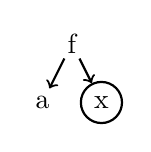
\begin{tikzpicture}[->,thick,scale=0.5, every node/.style={scale=1}]
          \tikzstyle{tnode}=[circle, inner sep=.5mm]
          \tikzstyle{var}=[ circle, inner sep=1mm,draw]
          \node[tnode] {f}
                    child {node[tnode] {a} }
                    child {node[var] {x} 
                    };
      \end{tikzpicture}, & \text{if}\ v=y \\%[5pt]
            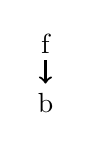
\begin{tikzpicture}[->,thick,scale=0.5, every node/.style={scale=1}]
                \tikzstyle{tnode}=[circle, inner sep=.5mm]
                \tikzstyle{var}=[ circle, inner sep=1mm,draw]
                \node[tnode] {f}
                            child {node[tnode] {b} }
                          ;
            \end{tikzpicture}, & \text{if}\ v= z
    \end{cases}
  \end{equation*}
  Подстановка c $Dom(\sigma) = \{y, z\}$
\end{minipage}
\hspace{.5cm}
\begin{minipage}[b]{0.3\linewidth}
\begin{center}
\begin{tikzpicture}[->,thick,scale=0.5, every node/.style={scale=0.5}
  , grow via three points={
      one child at (0,-2) and 
      two children at (.8,-2) and (-0.8,-2) 
  }]
     \tikzstyle{tnode}=[circle, inner sep=1.5mm]
     \tikzstyle{var}=[ circle, inner sep=1.5mm,draw]
     \def\rstep{5cm}
     \huge
         
    \begin{scope}[xshift= \rstep]
      \node[tnode] {f}
          child {node[tnode] {g} 
            child {node[tnode] {a} }
            child {node[var] {x} }
          }
          child[missing] {}
          child {node[tnode] {f}
                  child {node[var] {x} }
                  child {node[tnode] {a} }
          };
      \end{scope}
\end{tikzpicture}

Дерево после подстановки
\end{center}
\end{minipage}
\end{frame}

\begin{frame}
\begin{definition}[Более общая подстановка]
Подстановка $\sigma_0$ более общая, чем $\sigma$, если последнюю можно получить из первой путём специализации(сужения) более общей $\sigma_0$ на некоторых входах
\end{definition}
\vspace{1em}

Примеры:
\begin{itemize}
\item Подстановка $\{x\mapsto y, y\mapsto z\}$ более общая чем $\{x\mapsto 1, y\mapsto 1\}$, т.к. её можно сузить с помощью $z\mapsto 1$
%\item Подстановка $\{x\mapsto y, z\mapsto 1\}$ более общая чем $\{x\mapsto y, y\mapsto 1\}$, т.к. её можно сузить с помощью $y\mapsto 1$
\item Подстановки $\{y\mapsto 1\}$ и $\{z\mapsto y\}$ не являются более общими друг к другу
\end{itemize}
\end{frame}


\begin{frame}
\begin{definition}[Задача (синтаксической) унификации]
Даны два дерева с метапеременными. Необходимо подобрать наиболее общую подстановку-унификатор (\emph{most general unifier}, mgu) так, чтобы после её применения два дерева стали одинаковыми. Или же сказать, что mgu не существует.
\end{definition}
\end{frame}


\begin{frame}{Алгоритм синтаксической унификации}
\vspace{1em}
\textbf{Вход}: два дерева и стартовая подстановка $\sigma$.\\
\textbf{Выход}: подстановка-унификатор или её отсутствие.\\

Во время алгоритма синхронно обходим два дерева
\begin{itemize}
\item Унифицируем (мета)переменную $x\in Dom(\sigma)$, тогда надо вместо $x$ унифицировать $\sigma(x) \equiv \text{walk}(\sigma, x)$
\item Унифицируем (мета)переменную $x$ и дерево $\mathcal{V}$, но $\text{check}(\sigma,x,\mathcal{V})\equiv \text{false}$, т.е. не можем расширить подстановку  --- унификация не возможна
\item Если можем расширить подстановку, то выдаем ответ: $ \text{extend}(\sigma,x,\mathcal{V})$
\item Два разных функциональных символа -- унификация не возможна 
\item Иначе (два одинаковых функц. символа с одинаковой арностью $n$) мы попарно унифицируем аргументы, "протягивая" текущую подстановку через $n$ рекурсивных вызовов
\end{itemize}

\end{frame}


\begin{frame}{Упражнение 1}
Можно ли проунифицировать два выражения: $x+((2+f(y))+y)$ и  $f(y)+((2+x)+1)$?
\vspace{1em}

\begin{figure}[ht]
\begin{subfigure}{.35\textwidth}
\includegraphics[page=1,scale=1.3]{tikzpics/uniftrees2.pdf}
\end{subfigure}
\begin{subfigure}{.35\textwidth}
\includegraphics[page=2,scale=1.3]{tikzpics/uniftrees2.pdf}
\end{subfigure}
\begin{subfigure}{.25\textwidth}
Ответ: да
\begin{itemize}
\item $x \mapsto f(y)$ 
\item $y \mapsto 1$
\end{itemize}
\end{subfigure}
\end{figure}
\end{frame}

\begin{frame}[fragile]{Упражнение 2}
Проунифицировать $f(\alpha,\beta)$ и $f(l(\beta), n)$, где $\alpha,\beta$ -- метапеременные.
\vspace{1em}

\begin{minipage}{0.45\linewidth}
  \begin{center}
\includegraphics[page=1,scale=1.1]{tikzpics/uniftrees3.pdf}
  \end{center}
\end{minipage}\hspace{1cm}
\begin{minipage}{0.45\linewidth}
  \begin{center}
\includegraphics[page=2,scale=1.1]{tikzpics/uniftrees3.pdf}
  \end{center}
\end{minipage}
\vspace{1em}\pause

На выходе можно полученную подстановку записывать двумя способами:\\

\begin{minipage}[t]{0.45\linewidth}
\begin{center}
"Треугольная"
\begin{align*}
  \alpha &\mapsto f(\beta)\\
  \beta &\mapsto n
\end{align*} 
\end{center}
\end{minipage}\hspace{1cm}
\begin{minipage}[t]{0.45\linewidth}
\begin{center}
"Идемпотентная"
\begin{align*}
  \alpha &\mapsto f(n)\\
  \beta &\mapsto n
\end{align*} 
\end{center}
\end{minipage}
\end{frame}


\begin{frame}{Треугольная и идемпотентная подстановки}
\begin{center}
\begin{tabular}{ |>{\centering\arraybackslash}p{5cm}|>{\centering\arraybackslash}p{3cm}|>{\centering\arraybackslash}p{5cm}| } 
 \hline
 Треугольная & Название & Идемпотентная \\ \hline
 {$ \begin{aligned}
   \alpha &\mapsto f(\beta)\\
   \beta &\mapsto n
 \end{aligned}$}  & Пример & {$\begin{aligned}
   \alpha &\mapsto f(n)\\
   \beta &\mapsto n
 \end{aligned}  $} \\  \hline
 
 Зависит от значений других ключей & Значение $\sigma(x)$ & $\sigma(x)$ -- окончательный образ $x$ \\ \hline
  экспоненциальная* & Сложность операции \mlinline{walk} & константная*\\  \hline
  константная* & Сложность операции \mlinline{extend} & экспоненциальная*\\  \hline
\end{tabular}
\end{center}
\end{frame}


\begin{comment}
content

\begin{frame}[fragile]{Упражнение\uncover<3->{. Occurs check}}

Проунифицируйте  $f(x, y)$ и $y$.\pause

\begin{center}
Будет ошибка или
\begin{tikzpicture}[->,thick,scale=0.5, every node/.style={scale=0.5}
  , grow via three points={
      one child at (0,-2) and 
      two children at (.8,-2) and (-0.8,-2) 
  }]
     \tikzstyle{tnode}=[circle, inner sep=1.5mm]
     \tikzstyle{var}=[ circle, inner sep=1.5mm,draw]
     \def\rstep{5cm}
     \huge
      
      \begin{scope}[xshift=23cm]
        \node[tnode] (ffff) {f}
            child[missing] {}
            child {node[tnode] (gggg) {x} 
            }
            ;

        \draw [->,thick](ffff)
                to [out=-45,in=135] (1,-2)
                to [out=0,in=0]  (ffff.east); 
        \end{scope}
 \end{tikzpicture}?
\end{center}
\pause

\begin{definition}{Occurs check}
-- это проверка при расширении подстановки $\sigma$ c помощью $x\mapsto v$, что $x$ не входит в $walk(\sigma, v)$
\end{definition}
\end{frame}

\end{comment}